\documentclass[tikz]{standalone}
\usepackage{amsmath}
\usepackage{amssymb}
\usepackage{tikz}
\usepackage{pgfplots}
\usepackage{color}


\DeclareMathSizes{4}{4}{4}{4}
\usetikzlibrary{intersections}
\usetikzlibrary{patterns}
\usetikzlibrary{decorations.text}
\usetikzlibrary{decorations.markings}
\usetikzlibrary{arrows.meta}
\usetikzlibrary{arrows,decorations}
\usepgfplotslibrary{fillbetween}
\usetikzlibrary{calc}

\begin{document}

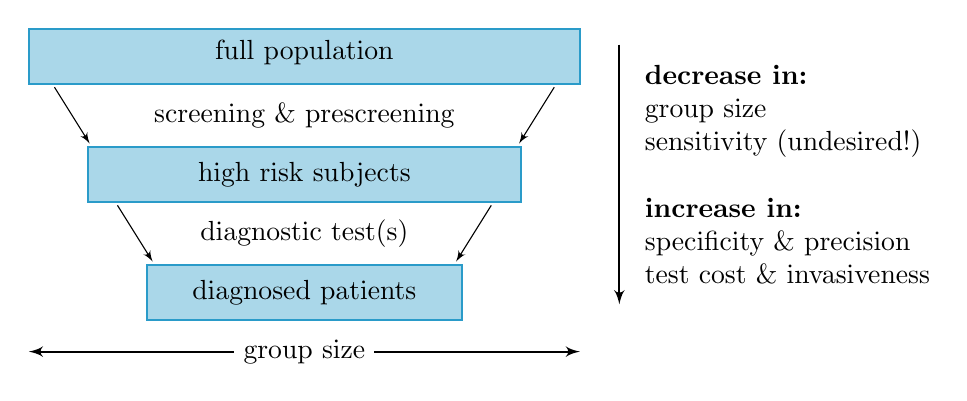
\begin{tikzpicture}

%\let scale=2

\draw[thick, draw=cyan!80!black, fill=cyan!80!black,fill opacity=0.4] (-3.5, 3.1) rectangle (3.5, 2.4);
\node[draw=none] at (0, 2.8) {full population};

\draw[-latex', shorten <=0.5mm, shorten >=0.5mm] (-3.2, 2.4) -- (-2.7, 1.6);
\draw[-latex', shorten <=0.5mm, shorten >=0.5mm] (3.2, 2.4) -- (2.7, 1.6);

\draw[thick, draw=cyan!80!black, fill=cyan!80!black,fill opacity=0.4] (-2.75, 1.6) rectangle (2.75, 0.9);
\node[draw=none, fill=white] at (0, 2.0) {screening \& prescreening};

\draw[-latex', shorten <=0.5mm, shorten >=0.5mm] (-2.4, 0.9) -- (-1.9, 0.1);
\draw[-latex', shorten <=0.5mm, shorten >=0.5mm] (2.4, 0.9) -- (1.9, 0.1);

\draw[thick, draw=cyan!80!black, fill=cyan!80!black,fill opacity=0.4] (-2.0, 0.1) rectangle (2.0, -0.6);
\node[draw=none, anchor=center] (blah) at (0, 1.25) {high risk subjects};
\node[draw=none, fill=white] at (0, 0.5) {diagnostic test(s)};
\node[draw=none, anchor=center] (blah) at (0, -0.25) {diagnosed patients};


\draw[latex'-latex', thick] (-3.5, -1) -- (3.5, -1);
\node[draw=none, fill=white] at (0, -1) {group size};

\draw[-latex', thick, shorten <=2mm, shorten >=2mm] (4, 3.1) -- (4, -0.6);
\node[draw=none, anchor=west, align=left] at (4.2, 1.25) {
	\textbf{decrease in:} \\
	group size \\
	sensitivity (undesired!) \\
	\ \\
	\textbf{increase in:} \\
	specificity \& precision \\
	test cost \& invasiveness
};

\end{tikzpicture}
\end{document}
